% ============================== Premable ======================================

\documentclass[tikz, border=0.005in]{standalone}
\usepackage{amsmath,amsfonts,amssymb, tikz, hyperref, fixltx2e, lscape}
\usetikzlibrary{backgrounds}
\usetikzlibrary{positioning}
\usetikzlibrary{shapes,arrows}
\usetikzlibrary{calc}
\tikzstyle{line} = [draw, -latex, thick]
\tikzstyle{term} = [draw, thick]
\renewcommand{\familydefault}{\sfdefault}
\definecolor{color1}{RGB}{51, 255, 153} % light green
\definecolor{color2}{RGB}{51, 153, 255} % light blue
\definecolor{color3}{RGB}{255, 230, 179} % light orange
\definecolor{color4}{RGB}{255, 153, 153} % light pink
\definecolor{color5}{RGB}{204, 235, 255} % light blue background
\definecolor{color6}{RGB}{216, 200, 118} % splitter
\definecolor{color7}{RGB}{94, 226, 218} % antenna
\definecolor{color8}{RGB}{241, 5, 182} % Mgr

% ============================== Document ======================================

\begin{document}

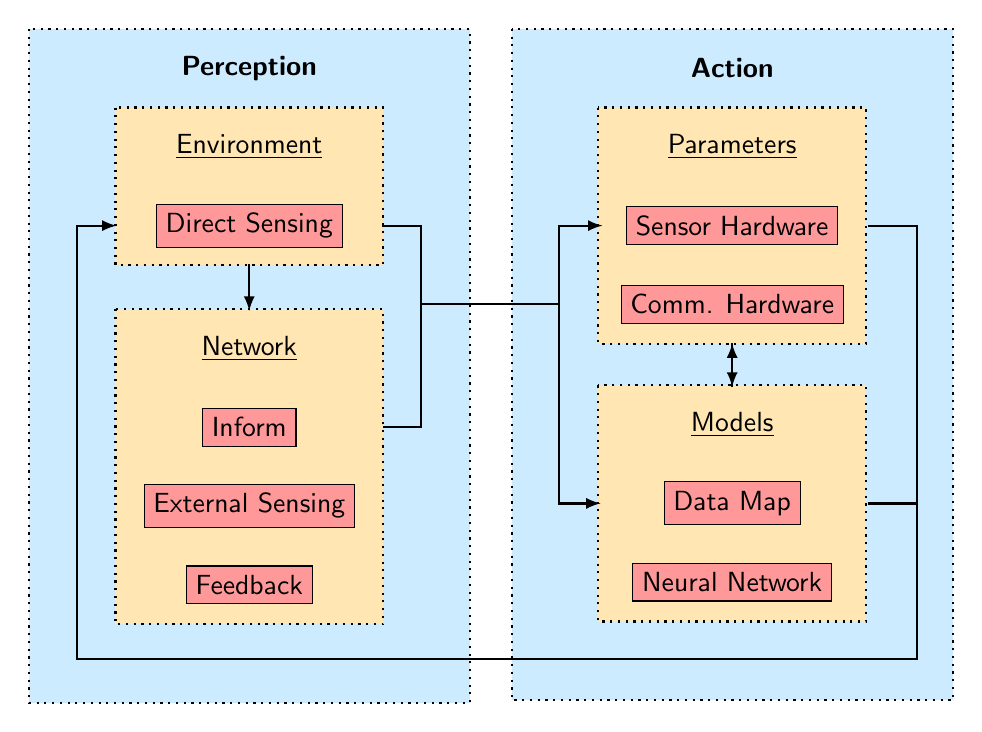
\begin{tikzpicture}

  % ============================ Perception ====================================

  \node (pc) {\bf Perception};
  \node[below of=pc] (env) {\underline{Environment}};
  \node[draw, fill=color4, below of=env] (ds) {Direct Sensing};
  \node[below=1cm of ds] (nw) {\underline{Network}};
  \node[draw, fill=color4, below of=nw] (if) {Inform};
  \node[draw, fill=color4, below of=if] (es) {External Sensing};
  \node[draw, fill=color4, below of=es] (fb) {Feedback};
  \begin{pgfonlayer}{background}
    \draw[thick,dotted,fill=color5] {
      ($(pc)+(-2.8,0.5)$) rectangle ($(fb)+(2.8,-1.5)$)
    };
  \end{pgfonlayer}
  \begin{pgfonlayer}{background}
    \draw[thick,dotted,fill=color3] {
      ($(env)+(-1.7,0.5)$) rectangle ($(ds)+(1.7,-0.5)$)
    };
  \end{pgfonlayer}
  \begin{pgfonlayer}{background}
    \draw[thick,dotted,fill=color3] {
      ($(nw)+(-1.7,0.5)$) rectangle ($(fb)+(1.7,-0.5)$)
    };
  \end{pgfonlayer}

  % ============================== Action ======================================

  \node[right=4.5cm of pc] (act) {\bf Action};
  \node[below of=act] (par) {\underline{Parameters}};
  \node[draw, fill=color4, below of=par] (sh) {Sensor Hardware};
  \node[draw, fill=color4, below of=sh] (ch) {Comm. Hardware};
  \node[below=1cm of ch] (mod) {\underline{Models}};
  \node[draw, fill=color4, below of=mod] (dm) {Data Map};
  \node[draw, fill=color4, below of=dm] (nn) {Neural Network};
  \begin{pgfonlayer}{background}
    \draw[thick,dotted,fill=color5] {
      ($(act)+(-2.8,0.5)$) rectangle ($(nn)+(2.8,-1.5)$)
    };
  \end{pgfonlayer}
  \begin{pgfonlayer}{background}
    \draw[thick,dotted,fill=color3] {
      ($(par)+(-1.7,0.5)$) rectangle ($(ch)+(1.7,-0.5)$)
    };
  \end{pgfonlayer}
  \begin{pgfonlayer}{background}
    \draw[thick,dotted,fill=color3] {
      ($(mod)+(-1.7,0.5)$) rectangle ($(nn)+(1.7,-0.5)$)
    };
  \end{pgfonlayer}

  % ============================= Connect ======================================
  \path[term]{
    ([xshift=0.5cm]ds.east)
    -| ([yshift=-1cm, xshift=1cm]ds.east)
    |- ([yshift=-1cm, xshift=2.75cm]ds.east)};
  \path[term]{
    ([xshift=1.1cm]if.east)
    -| ([yshift=-1cm, xshift=1cm]ds.east)};
  \path[line]{
    ([yshift=-1cm, xshift=2.75cm]ds.east)
    |- ([xshift=-0.3cm]sh.west)};
  \path[line]{
    ([yshift=-1cm, xshift=2.75cm]ds.east)
    |- ([xshift=-0.8cm]dm.west)};

  \path[term]{
    ([xshift=0.85cm]dm.east)
    -| ([xshift=1.47cm]dm.east)};
  \path[line]{
    ([xshift=0.38cm]sh.east)
    -| ([yshift=-5.5cm, xshift=1cm]sh.east)
    -| ([xshift=-1cm]ds.west)
    |- ([xshift=-0.5cm]ds.west)};
  \path[line]{
    ([yshift=-0.21cm]ds.south)
    -- ([yshift=0.2cm]nw.north)};
  \path[line]{
    ([yshift=-0.25cm]ch.south)
    -- ([yshift=0.2cm]mod.north)};
  \path[line]{
    ([yshift=0.2cm]mod.north)
    -- ([yshift=-0.25cm]ch.south)};

\end{tikzpicture}
\end{document}
